\subsection{Backend Implementering}

I det følgende afsnit gennemgåes implementerings detaljer omkring backendens controller klasser, samt BackEndController klassen på client siden. Alle controller klasserne er implementeret i C\#, da dette er sproget som anvendes i Asp.net Core. \\

\subsubsection{SaveController}
SaveController klassen inkluderer librariet Mircosoft.AspNetCore.MVC, dette gør det muligt, at anvende atributter til at definere hvilke Http metoder som funktionerne anvender eksempelvis HttpGet se figur x (Mangler ref).\\


\begin{figure}[H]
\centering
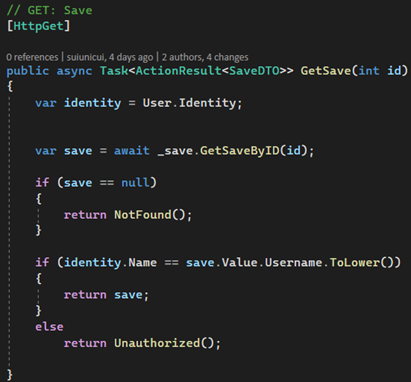
\includegraphics[width = \textwidth]{02-Body/Images/Backend_Code_GetSave.PNG}
\caption{Code snippet af HttpGet metode som modtager et id og retunere et SaveDTO object til clienten}
\label{fig:Arkitektur-Backend-Code-GetSave}
\end{figure}

Librariet gør det ligeledes muligt at retunere ActionResults, som kan indeholde objekter og en status kode eller blot en status kode, hvis noget går galt. Alle funktionerne er async og retunerer en Task, hvilket gør at der er tale om asynkrone funktioner, der først retunerer en værdi når dataen er klar. Dette gør også at clienten kan klare andre opgaver ind til dataen er klar.
SaveController inkludere også Microsoft.AspNetCore.Authorization librariet, som bidrager med funktionalitet til kun at tilade kald, fra en korrekt bruger med Atributten [Authorize]. Da der kun findes en type af identiteter nemlig en helt normal bruger, som har adgang til alle endpoints, skal der findes en måde at sikre at brugeren kun kan tilgå sine egne data. Derfor gøres brug af User.Identity, kan ses på figur 10. Dette anvendes til at hente Claims om den User, som tilhører den nuværende action, som så kan bruges til at tjekke om brugeren har lov til at hente det pågældende gemte spil.\\
    

\subsubsection{UserController}

UserController klassen minder meget om SaveController klassen, den gør ligeledes brug af Libraries Microsoft.AspNetCore.MVC og Microsoft.AspNetCore.Authorize. På figur x (mangler ref til figur) ses Login funktionen.

\begin{figure}[H]
\centering
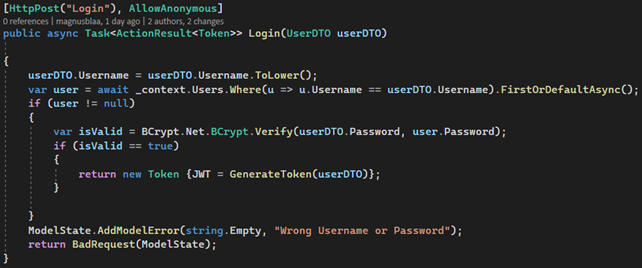
\includegraphics[width = \textwidth]{02-Body/Images/Backend_Code_Login.PNG}
\caption{Code snippet af HttpPost metode som modtager et UserDTO object og retunerer en JWT hvis brugeren findes og password’et er korrekt}
\label{fig:Arkitektur-Backend-Code-Lgoin}
\end{figure}

Her tilføjes endnu en atrribut AllowAnonymous, da login skal være et anonymt kald, fordi brugeren endnu ikke er logget ind på clienten. Hvis brugeren findes og kodeordet er korrekt retuneres en ny JWT.\\

\subsubsection{BackEndController Client}
BackEndControlleren indeholde som det blev nævnt i backend Design afsnittet (Mangler Ref) et HttpClient objekt til at håndtere http request/response, og et Token objekt til at holde på den modtagne JWT.
Et klasse diagram over BackEndControlleren kan ses på figur x.\\

\begin{figure}[H]
\centering
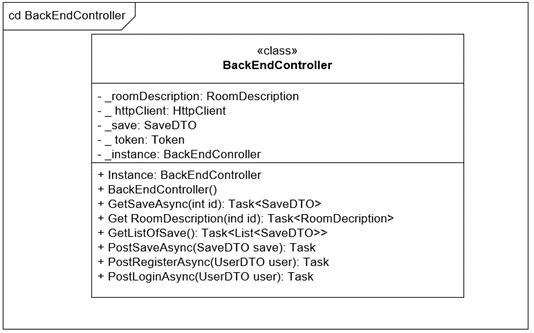
\includegraphics[width = \textwidth]{02-Body/Images/Backend_klasse_BackEndController.PNG}
\caption{klasse diagram af BackEndController}
\label{fig:Arkitektur-Backend-Klasse-BackEndController}
\end{figure}

For at sikre at der kun findes en JWT i programmet ad gangen, skal BackEndController implementeres klassen som en singleton, hvilket vil sige at der kun eksiterer en enkelt instance i hele programmet, som der er global adgang til. På den måde sikres det nemlig at BackEndController altid indeholder den korrekte JWT, uanset hvor henne i programmet der laves en request fra. Uden dette ville JWT nemlig kun være sat inde i det scope, hvor der blev logget ind eller en bruger blev registreret fra, altså der hvor den nuværende instance af BackendControlleren eksiterer. Funktionerne her er ligeledes asynkrone.\\


\subsubsection{Konlusion}

Funktionerne i backend controller klasserne samt funktionerne på clientens BackEndController er implementeret som asynkrone funktioner, der først retunerer en værdi når resourcen som efterspørges er klar. Client klassen er implementeret som en singleton for at holde styr på den aktuelle JWT.

\newpage
